In this section we will go over examples of lattice code and discuss the outputted result.

\subsection{Basic Graphs}
Our first implementation is a simple graph that exposes the features that we have created.

\begin{figure}[H]
    \centering
    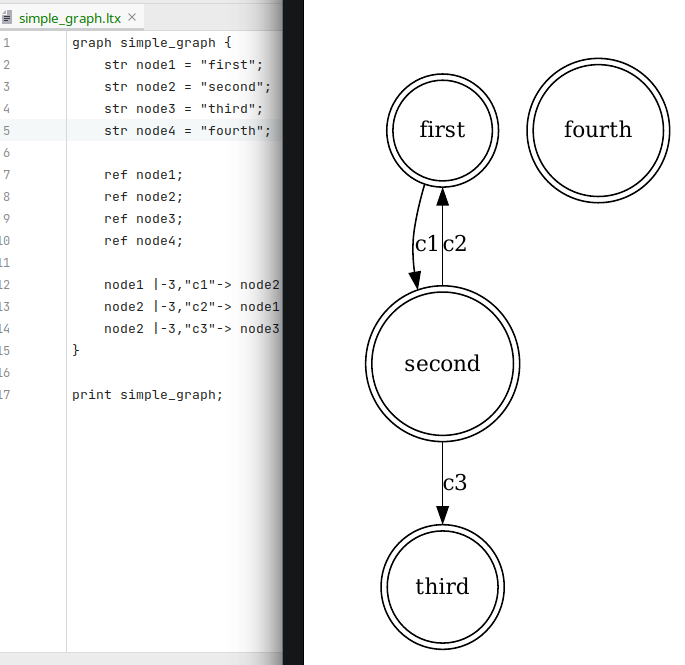
\includegraphics[width=12cm]{figures/worked_example_graphs/simple-graph}
    \caption{A simple graph demonstrating all visual functionality}
    \label{fig:basic_graph_visualisation}
\end{figure}

There is very little to discuss here, as this is simply a demonstration that all the layers of the compiler are
functioning properly.

\subsection{Grid Graph}
